\documentclass[fleqn,10pt]{wlscirep}
\usepackage[utf8]{inputenc}
\usepackage[T1]{fontenc}
\usepackage{lineno}
\usepackage{siunitx}
\usepackage{listings}
\usepackage{tikz}
\usetikzlibrary{positioning, arrows.meta}
\usepackage{graphicx}
\usepackage{ulem}  % for striking through text
\usepackage[table]{xcolor}
\usepackage{glossaries}
\usepackage{csvsimple}
\usepackage{bm} % Bold math
\usepackage{todonotes}
\usepackage[version=4]{mhchem}
\usepackage{eurosym}
\usepackage[author={Bobby Xiong}]{pdfcomment}
\usepackage{makecell} % for line breaks in table cells
\usepackage{pdflscape}
\usepackage{array}
\glsdisablehyper % Disable hyperlinks for glossary entries
\let\autocite\cite
\linenumbers

%%% Acronyms

\newacronym{api}{API}{Application Programming Interface}
\newacronym{osm}{OSM}{OpenStreetMap}
\newacronym{entsoe}{ENTSO-E}{European Network of Transmission System Operators for Electricity}
\newacronym[plural=tso,firstplural=Transmission System Operators (TSOs)]{tso}{TSO}{Transmission System Operator}
\newacronym{ac}{AC}{Alternating Current}
\newacronym{dc}{DC}{Direct Current}
\newacronym{rmse}{RMSE}{Root Mean Square Error}
\newacronym{odbl}{ODbL}{Open Data Commons Open Database License}


\newcommand{\fixedcolorbox}[2]{%
  \begingroup
  \setlength{\fboxsep}{0pt}% No padding
  \colorbox{#1}{\strut#2}% Ensure line height doesn't change
  \endgroup
}
\newcommand{\colorcode}[1]{\colorbox{gray!20}{\lstinline|#1|}}

% Column type center:
\newcolumntype{C}[1]{>{\centering\arraybackslash}p{#1}}

%%% Acronyms end

\title{Modelling the high-voltage grid using open data for Europe and beyond}

\author[1,*]{Bobby Xiong}
\author[2]{Davide Fioriti}
\author[1]{Fabian Neumann}
\author[1]{Iegor Riepin}
\author[1]{Tom Brown}
\affil[1]{Technische Universität Berlin, Department of Digital Transformation in Energy Systems (Institute of Energy Technology), Berlin, Germany}
\affil[2]{Università di Pisa, Department of Energy Systems, Territory and Construction Engineering, Pisa, Italy}

\affil[*]{corresponding author: Bobby Xiong (\href{mailto:xiong@tu-berlin.de}{xiong@tu-berlin.de})}


\begin{abstract}
% \pdfcomment{This is a manuscript template for Data Descriptor submissions to \emph{Scientific Data} (\href{http://www.nature.com/scientificdata}{http://www.nature.com/scientificdata}). The abstract must be no longer than 170 words, and should succinctly describe the study, the assay(s) performed, the resulting data, and the reuse potential, but should not make any claims regarding new scientific findings. No references are allowed in this section.}
This paper provides the background, methodology and validation for constructing a representation of the European high-voltage grid, including and above 200 kV, based on public data provided by OpenStreetMap. The model-independent grid dataset is published under the Open Data Commons Open Database (ODbL 1.0) licence and can be used for large-scale electricity as well as energy system modelling. The dataset and workflow are provided as part of PyPSA-Eur -- an open-source, sector-coupled optimisation model of the European energy system. By integrating with the codebase for initiatives such as PyPSA-Earth, the value of open and maintainable high-voltage grid data extends to the global context. By accessing the latest data through the the Overpass turbo API, the dataset can be easily reconstructed and updated within minutes. To assess the data quality, this paper further compares the dataset with official statistics and representative model runs using PyPSA-Eur based on different electricity grid representations.
\end{abstract}
\begin{document}

\flushbottom
\maketitle
%  Click the title above to edit the author information and abstract

\thispagestyle{empty}

% \pdfcomment{Please note: Abbreviations should be introduced at the first mention in the main text – no abbreviations lists or tables should be included. Structure of the main text is provided below.}
\section*{Background \& Summary}
% \pdfcomment{(700 words maximum) An overview of the study design, the assay(s) performed, and the created data, including any background information needed to put this study in the context of previous work and the literature. The section should also briefly outline the broader goals that motivated the creation of this dataset and the potential reuse value. We also encourage authors to include a figure that provides a schematic overview of the study and assay(s) design. The Background \& Summary should not include subheadings. This section and the other main body sections of the manuscript should include citations to the literature as needed.}
Energy system models are indispensable tools in today's world in order to understand the complex interactions between energy sources, technologies, policies, and markets. They are used by researchers, industry and policy makers to enable informed decision-making in the transition to a net-zero energy system. However, conclusions drawn from such models are only as good as the underlying data and assumptions. Especially the representation of existing energy infrastructure, such as the electricity grid, can have a deciding impact on future investments derived from such models.\autocite{horschRoleSpatialScale2017} While \glspl{tso} have their own information on the high-voltage grid, this data is often not publicly available to the level of detail needed for academic research purposes. Official institutions like the \gls{entsoe} provide an online map \autocite{entso-eENTSOETransmissionSystem} of the European high-voltage grid. There are however, several limitations typical for these sources: i) there is no underlying, topologically connected dataset, ii) it is not released under an open licence, iii) nor updated frequently, and iv) its geographic detail is limited or highly stylised.

There are previous projects that have modelled the European high-voltage grid or its parts based on \gls{osm} data. Some institutions provide data for particular regions, however all of them come with their individual limitations: While the most trustworthy data comes from \acrshortpl{tso} themselves, they are --- with few regional exceptions \autocite{50hertzStaticGridModel2022} --- not georeferenced \autocite{jaoStaticGridModel2023} or do not cover the entirety of Europe. Datasets from previous academic projects \autocite{egererElectricitySectorData2014,hutcheonUpdatedValidatedPower2013,medjroubiOpenDataPower2017} are either very complex to reproduce or have not been updated for close to a decade. An overview of notable projects and datasets is listed in Table \ref{tab:network_projects}. Proven to be a reliable public data source, we make use of \acrshort{osm} to introduce a transparent workflow in order to create a representation of the European high-voltage grid. On the lack of updates of existing datasets, there are two main advantages of our work compared to previous initiatives. First, our approach uses the \acrshort{osm} Overpass turbo \gls{api}\autocite{raiferOverpassTurbo2024} that always allows to retrieve the latest \acrshort{osm} data. Second, an active \acrshort{osm} community as well as a large user base of PyPSA-Eur and integration into automated workflows mean frequent updates and validation of processed data. Debugging can be easily done with the help of the open source project OpenInfraMap \autocite{garrettOpenInfrastructureMap2024} which renders the \gls{osm} energy infrastructure on an interactive map. Finally, the entire workflow is developed in Python and may hence be more accessible than other implementations which require external dependencies (e.g. SQL databases, commercial software, Java).\autocite{wiegmansGridKitExtractENTSOE2016}

Compared to previous implementations in the global modal PyPSA-Earth,\autocite{parzenPyPSAEarthNewGlobal2023} we significantly improve the work in speed and data quality by taking advantage of the topological, electrical and geographical information available for Europe in \gls{osm}. Given the generic structure of the developed workflow, it can be easily applied to other regions and fed back to the global PyPSA-Earth project. However, the output will directly depend on the \acrshort{osm} data quality for a particular region (e.g. whether data on the substation's geometric footprint is available). To fill in missing data, we introduce cleaning process that yields a representation of the European high-voltage grid. 
We benchmark the processed data against country-level statistics provided by ENTSO-E, concluding that \acrshort{osm} data coverage of the European high-voltage grid is high or even close to complete. These improvements will also contribute to the quality of transmission grids modelled on a global scale in PyPSA-Earth. 
\section*{Methods}
% \pdfcomment{The Methods should include detailed text describing any steps or procedures used in producing the data, including full descriptions of the experimental design, data acquisition assays, and any computational processing (e.g. normalization, image feature extraction). See the detailed section in our submission guidelines for advice on writing a transparent and reproducible methods section. Related methods should be grouped under corresponding subheadings where possible, and methods should be described in enough detail to allow other researchers to interpret and repeat, if required, the full study. Specific data outputs should be explicitly referenced via data citation (see Data Records and Citing Data, below).
% Authors should cite previous descriptions of the methods under use, but ideally the method descriptions should be complete enough for others to understand and reproduce the methods and processing steps without referring to associated publications. There is no limit to the length of the Methods section. Subheadings should not be numbered.}
PyPSA-Eur is a spatially and temporally highly resolved, open-source, sector-coupled linear optimisation model that covers the European continent.\autocite{horschPyPSAEurOpenOptimisation2018} The model is build on top of the open-source toolbox PyPSA \autocite{brownPyPSAPythonPower2018} and is suited for operational as well as expansion studies (transmission, generation, and storages). The model includes a stock of existing power plants (processed with the tool powerplanmatching\autocite{gotzensPerformingEnergyModelling2019}) as well as renewable potentials and availability time series (processed with atlite\autocite{hofmannAtliteLightweightPython2021}).
Throughout the last decade, PyPSA-Eur has gained a large user base from academia, industry, and policy makers alike and has been used in a variety of studies.\autocite{neumannPotentialRoleHydrogen2023,victoriaSpeedTechnologicalTransformations2022,brownUltralongdurationEnergyStorage2023,glaumOffshorePowerHydrogen2024,riepinMeansCostsSystemlevel2024,rahdanDistributedPhotovoltaicsProvides2024,grochowiczUsingPowerSystem2024,transnetbwStromnetz2050Studie2022} Other open-source models exist, one notable being OSeMOSYS Global,\autocite{barnesOSeMOSYSGlobalOpensource2022} however it lacks the detailed geographical as well as electrical representation of the transmission grid that PyPSA-Eur provides. With the integration into PyPSA-Eur, we also enable compatibility with additional functions already implemented into the model, such as, but not limited to, the option to enable dynamic line rating\autocite{glaumLeveragingExistingGerman2023} and adding projects under planning (e.g. European Ten-Year Network Development Plan\autocite{entso-eTenYearNetworkDevelopment2020} and the German Network Development Plan\autocite{bnetzaBestaetigungNetzentwicklungsplanStrom2024}).

\begin{figure}[h!]
    \centering
    \resizebox{0.85\textwidth}{!}{
        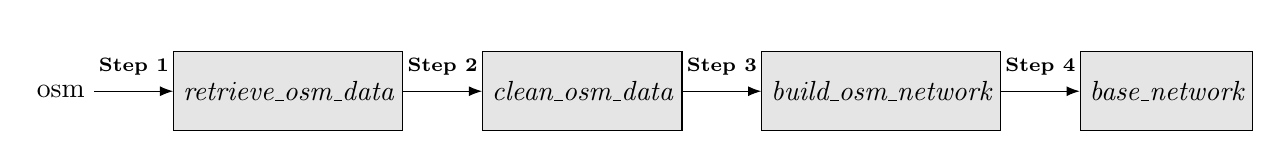
\begin{tikzpicture}[node distance=1cm, every node/.style={draw, minimum height=1cm, minimum width=0cm, align=center}, >=Latex]
            % Nodes
            \node[draw=none] (osm) {\gls{osm}};
            \node[fill=gray!20, font=\itshape] (retrieve) [right=of osm] {retrieve\_osm\_data};
            \node[fill=gray!20, font=\itshape] (clean) [right=of retrieve] {clean\_osm\_data};
            \node[fill=gray!20, font=\itshape] (build) [right=of clean] {build\_osm\_network};
            \node[fill=gray!20, font=\itshape] (base) [right=of build] {base\_network};

            % Arrows and Labels
            \draw[->] (osm) -- (retrieve) node[midway, above, draw=none, font=\scriptsize, yshift=-2mm] {\textbf{Step 1}};
            \draw[->] (retrieve) -- (clean) node[midway, above, draw=none, font=\scriptsize, yshift=-2mm] {\textbf{Step 2}};
            \draw[->] (clean) -- (build) node[midway, above, draw=none, font=\scriptsize, yshift=-2mm] {\textbf{Step 3}};
            \draw[->] (build) -- (base) node[midway, above, draw=none, font=\scriptsize, yshift=-2mm] {\textbf{Step 4}};
        \end{tikzpicture}
    }
    \caption{Process diagram for creating the European high-voltage grid from \gls{osm} data, representing the snakemake rules.}
    \label{fig:osm_process}
\end{figure}

PyPSA-Eur is managed by a workflow management system called Snakemake. \autocite{molderSustainableDataAnalysis2021} Its modular structure enables the addition of new model functionalities and data sources, these can then be toggled using a configuration file. We split the construction of the high-voltage grid into four steps and add them into the existing workflow. We also use the model for validation purposes (see section Technical Validation). While the dataset and its reconstruction is built into PyPSA-Eur, it has the potential to be used in other energy system models, too. To obtain a functioning, topologically connected representation of the European high-voltage grid based on \gls{osm} data, we take the following steps (see Figure \ref{fig:all_steps} for an application to an example region).

\begin{figure}[!htbp]
    \centering
    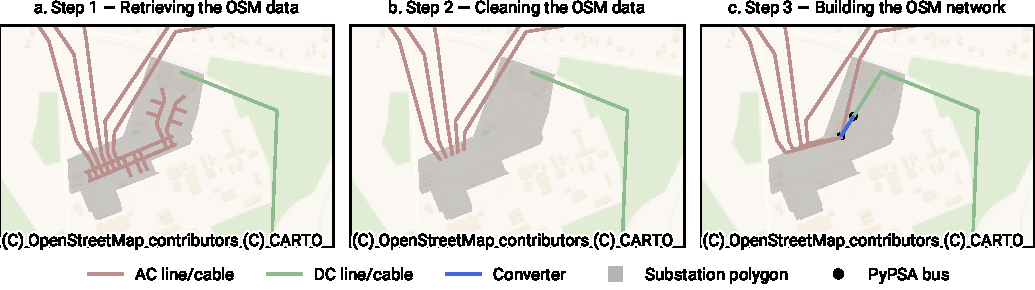
\includegraphics{figures/fig_all_steps.pdf}
    \caption{Illustration of the steps to create a PyPSA-ready network from \gls{osm} data. \textit{Note that Step 4 does not make changes to the topology and is hence omitted from this illustration.}}
    \label{fig:all_steps}
\end{figure}

\subsection*{Step 1 --- Retrieving the \gls{osm} data}
In \gls{osm}, geographical data is stored in `nodes', `ways', and `relations'. Being the simplest data type, nodes are defined by coordinates and associated parameters. Ways are geometric line strings that connect a set of nodes. Relations can contain nodes, ways, a combination of either or other relations. \autocite{medjroubiOpenDataPower2017} For the purpose of this work, we extract ways for obtaining the outline of substations and \acrshort{ac} power lines and cables. To obtain \acrshort{dc} projects (usually cables, hereafter refered to as \acrshort{dc} links), we use relations. There are two main reasons for this differentiation: i) relations are the more complex data type, coverage for \acrshort{ac} lines and cables is still scarce for Europe, whereas for \acrshort{dc} links, given that there are much fewer of them in Europe, coverage is close to complete (see Table \ref{tab:dc_links}); ii) Some \acrshort{dc} links contain multiple components, accessing relations allows us to efficiently aggregate and simplify the links for the purpose of static energy system modelling.
First, we retrieve the raw data using the Overpass turbo \gls{api}\autocite{raiferOverpassTurbo2024} (Figure \ref{fig:all_steps}.a). Specifically, we query the \gls{osm} database for electricity grid related features (see Table \ref{tab:overpass_queries}). Note that Overpass turbo has a limit on the size and number of requests for each query and provides the \gls{api} under a fair use policy. To avoid unnecessary load and re-use of data, we provide a prepared transmission grid for for download via Zenodo. \autocite{xiongPrebuiltElectricityNetwork2024}

\subsection*{Step 2 --- Cleaning the \gls{osm} data}
While \gls{osm} provides a rich dataset, it is not directly usable for energy system modelling. Next to geospatial coordinates, \gls{osm} includes tags that provide feature-specific additional information. Depending on the individual feature, data may however contain noise, be incomplete, or inconsistent. After importing the retrieved raw data into a pandas dataframe,\autocite{mckinneyDataStructuresStatistical2010} we apply a series of steps including heuristics to clean and fill in the missing information (see example in Table \ref{tab:aclines_example1}). We then use the power of geopandas\autocite{jordahlGeopandasGeopandasV02020} to perform geospatial operations (including but not limited to spatial joins, intersections, buffering, etc.).

\subsubsection*{Substations and transformers}
To obtain the set of substations, we filter for substations with a voltage level within the scope of interest, i.e. between \acrshort{ac} \SI{200}{\kilo\volt} and \SI{750}{\kilo\volt}. Where available, we extract the polygon shape of the substations, stored in the element's geometry. This allows us to differentiate between internal and external grid components. 
Note that information on transformers are not extracted from \acrshort{osm}, as i) we cannot adequately evaluate their coverage and ii) this data is not sufficient to create a topologically connected network. Instead, we use a needs-based approach, i.e. adding a single transformer of \SI{2000}{\mega\watt} between buses of different voltages within the perimeter of the same substation. This is in line with previous approaches to obtain the ENTSO-E map based transmission grid.\autocite{horschPyPSAEurOpenOptimisation2018}

\subsubsection*{\acrshort{ac} lines and cables} In a first step, we clean the tag columns to only contain the correct data type and unit, as shown in Table \ref{tab:aclines_params} for \acrshort{ac} power lines and cables. The minimum parameters that need to be given for a particular line or cable are `voltage' (in \si{\volt}) and `power' (string: `line' or `cable').
% 
\begin{table}[ht]
    \centering
    \begin{tabular}{|l|c|c|}
    \hline
    \textbf{Tag} & \textbf{Data type} & \textbf{Example} \\
    \hline
    cables & numeric & 9 \\
    \hline
    circuits & numeric & 3 \\
    \hline
    frequency & numeric & \SI{50}{\hertz} \\
    \hline
    power & string & line \\
    \hline
    voltage & numeric & \SI{380000}{\volt} \\
    \hline
    \end{tabular}
    \caption{Key tags/parameters for \acrshort{ac} power lines and cables.}
    \label{tab:aclines_params} 
\end{table}

We filter for the entries with a voltage level including and above \acrshort{ac} \SI{200}{\kilo\volt}. While data for the mid- to low-voltage grid is also partially available in \gls{osm}, public statistics are scarce, making validation of such data difficult. As not all entries contain clean or complete data, we make heuristic assumptions to fill in the gaps, as illustrated in Tables \ref{tab:aclines_example1} and \ref{tab:aclines_example2}. 

\begin{table}[!htbp]
    \centering
    \begin{tabular}{|l|c|c|c|c|c|c|}
    \hline
    \textbf{line id} & \textbf{cables} & \textbf{circuits} & \textbf{frequency} (Hz) & \textbf{type} & \textbf{voltage}  (V) \\
    \hline
    way/1 &  & 2 & 50 & cable & \SI{380000}{} \\
    \hline
    way/2 & 3 &  & 50 & cable & \SI{380000}{} \\
    \hline
    way/3 & 9 & 1;2 & 50 & line & \SI{380000}{}; \SI{220000}{} \\
    \hline
    way/4 & 9 & 3 & 50; 50 & line & \SI{380000}{}; \SI{220000}{} \\
    \hline
    way/5 & 8 &  & 50 & line & \SI{110000}{}; \SI{220000}{} \\
    \hline
    way/6 &  &  & 50 & cable & \SI{300000}{}\\
    \hline
    \end{tabular}
    \caption{Illustrative example of \acrshort{ac} lines and cables input data.}
    \label{tab:aclines_example1}
\end{table}

\begin{table}[!htbp]
    \centering
    \begin{tabular}{|l|c|c|c|c|c|}
    \hline
    \textbf{line id} & \textbf{circuits} & \textbf{frequency (Hz)} & \textbf{type} & \textbf{voltage (V)} \\
    \hline
    way/1 & 2 & 50 & cable & \SI{380000}{} \\
    \hline
    way/2 & \cellcolor{yellow!50}1 & 50 & cable & \SI{380000}{} \\
    \hline
    way/3-1 & \cellcolor{yellow!50}1 & 50 & line & \cellcolor{yellow!50}\SI{380000}{} \\
    \hline
    way/3-2 & \cellcolor{yellow!50}2 & 50 & line & \cellcolor{yellow!50}\SI{220000}{} \\
    \hline
    way/4-1 & \cellcolor{yellow!50}1 & \cellcolor{yellow!50}50 & line & \cellcolor{yellow!50}\SI{380000}{} \\
    \hline
    way/4-2 & \cellcolor{yellow!50}1 & \cellcolor{yellow!50}50 & line & \cellcolor{yellow!50}\SI{220000}{} \\
    \hline
    \sout{way/5-1} & \cellcolor{yellow!50}\sout{1} & \sout{50} & \sout{line} & \cellcolor{yellow!50}\sout{\SI{110000}{}} \\
    \hline
    way/5-2 & \cellcolor{yellow!50}1 & 50 & line & \cellcolor{yellow!50}\SI{220000}{} \\
    \hline
    way/6 & \cellcolor{yellow!50}1 & 50 & cable & \SI{300000}{}\\
    \hline
    \end{tabular}
    \caption{Illustrative example of \acrshort{ac} lines and cables after cleaning. Changes highlighted in yellow.}
    \label{tab:aclines_example2} 
\end{table}

For each line or cable we use the most specific information available that the data provides. In a three-phase \acrshort{ac} high-voltage system, we assume three cables to form an \acrshort{ac} circuit (e.g. way/2).\autocite{kirschenPowerSystemsFundamental2024} If a way contains multiple data points split by semicolons (i.e. transmission lines sharing overhead line routes), we split the entries into individual lines, accordingly. In this process, we preserve the original \gls{osm} identifier and its associated geometries. We add a numbered suffix after the split to maintain unique line ids (e.g. way/3 becomes way/3-1 and way/3-2). The given electric parameters are mapped according to the semicolon splits. In some cases however, where the number of data points across columns is not equal (e.g. way/4 and way/5), we make the following assumption: we take the floor of the number of circuits divided by the number of entries in the voltage column. In the absence of better information, this may lead to an underestimation of the real number of circuits. If no information on cables nor circuits are available, we assume a single circuit, provided that a voltage level is given (e.g. way/6). Finally, we remove all ways which represent bus bars and lines which are located fully inside of a substation outline (Figure \ref{fig:all_steps}.b), as they are considered internal elements of the substation and provide no additional information for the purpose of static analyses.
\subsubsection*{DC links and converters}
Due to their distinct electrical properties, we treat \acrshort{dc} links differently from \acrshort{ac} lines and cables. To avoid double counting, we remove all \acrshort{dc} links from the original way queries. Instead, we query the \gls{osm} database for relations that contain \acrshort{dc} links. As data on \acrshort{dc} projects are widely available and because there are fewer of them,\autocite{entso-eENTSOETransmissionSystem,pierriChallengesOpportunitiesEuropean2017} we contribute to the \gls{osm} database by adding missing parameters such as the nominal rating and voltage level. This signifies the ease of data improvements with OSM for the benefit of all. In order for future \acrshort{dc} projects to be traced by our workflow, the following tags are required: `route' = `power', `frequency' = 0, and `rating' in `X MW' format. \acrshort{dc} components need to be correctly linked in the \acrshort{osm} database as member (either `cable' or `line') of the parent relation, respectively.

\begin{figure}[!htbp]
    \centering
    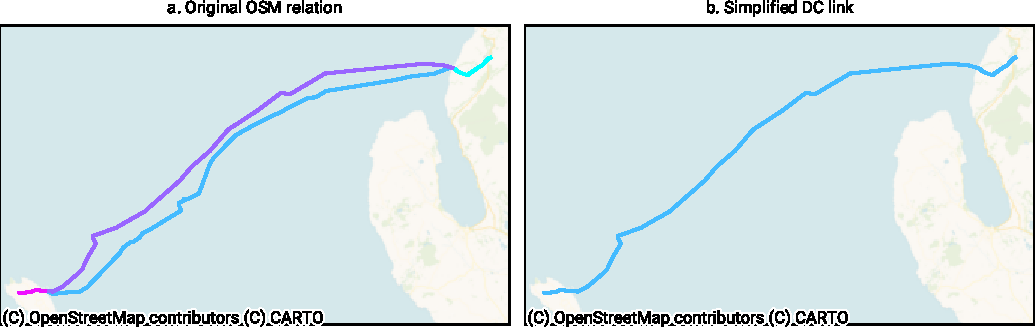
\includegraphics{figures/fig_dc_example.pdf}
    \caption{Example -- Simplification of a \acrshort{dc} link relation: Moyle interconnector (Scotland - Northern Ireland), \acrshort{osm} relation ID \href{https://www.openstreetmap.org/relation/6914309}{6914309}. \textit{Different colors show the four segments, i.e. ways that compose the \acrshort{osm} relation.}}
    \label{fig:dc_example}
\end{figure}

Note some relations contain multiple \acrshort{dc} link segments or components (e.g. converter stations or grounding), these are simplified into a single line with the sum of their nominal ratings. Figure \ref{fig:dc_example} shows an example of how the Moyle interconnector from Northern Ireland to Scotland (Figure \ref{fig:dc_example}.a) is simplified (Figure \ref{fig:dc_example}.b). In this simplification, we preserve original end points of the \acrshort{dc} link and the longest connected path. In PyPSA, converters are modelled as links connecting two buses. In analogy to how transformers are introduced to the network ex-post. i.e. connecting the terminals of the \acrshort{dc} link, where the converter stations are also located on \acrshort{osm} and the closest \acrshort{ac} bus in the transmission grid. As such, we guarantee that \acrshort{dc} links are always topologically connected.

\subsection*{Step 3 --- Building the \gls{osm} network}
\begin{figure}[!htbp]
    \centering
    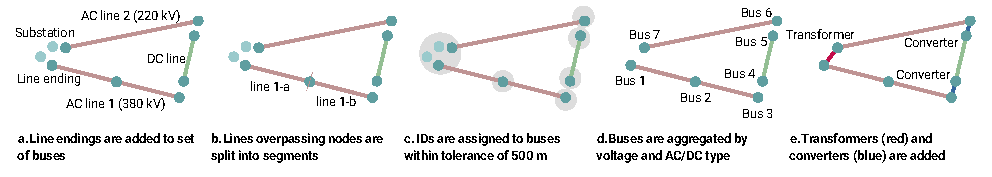
\includegraphics[width=\linewidth]{figures/fig_build_osm_network.pdf}
    \caption{Illustration of building a topologically connected grid.}
    \label{fig:build_osm_network}
\end{figure}

After having obtained a cleaned dataset, we need to ensure that the grid components are topologically and electrically connected. For this purpose, we propose a complete graph-based structure, i.e. buses/substations are connected by \acrshort{ac} and \acrshort{dc} lines, as well as converters and transformers. We introduce the following procedure, illustrated in Figure \ref{fig:build_osm_network}.

First, we add the endpoints of both \acrshort{ac} and \acrshort{dc} lines to the set of buses (Figure \ref{fig:build_osm_network}.a). This step ensures that each line has two corresponding buses to which it is initially connected. Note that this may introduce potential duplicates of buses beyond those already present --- which we will take care of later. Next, we take of long lines that are overpassing (multiple) substations. Here we assume that in reality, the substation is electrically connected to the overpassing line. To achieve this, we split the original line into the subsegments between the intersecting nodes and add a suffix to its original identifier (Figure \ref{fig:build_osm_network}.b), to i) preserve the uniqueness of each line and ii) still allow for tracing back the line on \acrshort{osm} or OpenInfraMap.\autocite{garrettOpenInfrastructureMap2024} We update the endpoints of the split lines, accordingly. Third, we cluster all buses within a radius of \SI{5000}{\meter}. We do this for several reasons, i) to avoid duplicates of buses that represent the same substation in reality, ii) to improve the computational efficiency of the model and iii) to improve the topological connectedness of the obtained network. In an interative procedure, buses within the given radius are assigned the same ID (Figure \ref{fig:build_osm_network}.c). Fourth, we cluster all buses assigned to the same station ID and \acrshort{ac}/\acrshort{dc} type. For each of the clusters, a bus is created. Connected lines are remapped, accordingly (Figure \ref{fig:build_osm_network}.d). Finally, we ensure that all given components are correctly electrically connected, i.e. \acrshort{ac} buses of different voltage levels at the same substation are linked by transformers, \acrshort{dc} buses which represent endpoints of \acrshort{dc} lines are connected to the closest \acrshort{ac} bus through converters (Figure \ref{fig:build_osm_network}.e) of equal nominal rating, respectively.

% \begin{itemize}
%     \item First, we enhance the original substations dataset by including the endpoints of both \acrshort{ac} and \acrshort{dc} lines. This step ensures consistency between the substation and line datasets by guaranteeing that each line has a corresponding substation at its endpoint. However, as shown in Fig. \ref{fig:step_3}, this process can introduce additional duplicate substations beyond those already present, which need to be addressed.
%     \item Second, as \gls{osm} data are not model-ready, we need to ensure the connectivity of long lines that may pass through multiple substations. When a line path overpasses a substation, the line is divided into two segments thus ensuring the so-called overpassing node is connected to the whole system. In Fig. \ref{fig:step_3}, `line B' is divided into segments `a' and `b' to ensure the connection of the overpassing bus to the whole system.
%     \item Third, we cluster the buses within a radius of \SI{5000}{\meter} to avoid duplicated substations and improve the computational efficiency of the model. This is done by an iterative procedure that assign a bus ID to each susbtation and its neighbours iteratively. If a neighbour within the radius is already assigned an ID, then its value is set to the current bus; otherwise a new ID is generated. This step is repeated for \acrshort{ac} and \acrshort{dc} substations, hence ensuring different IDs for each type. By doing so, the same ID may be assigned to substations with multiple voltage values.
%     \item Forth, resulting substations are clustered by ID, voltage level and AC/DC status and for each cluster an electrical bus is created. Fig. \ref{fig:step_3} shows an example of the procedure.
%     \item Fifth, to properly represent the network, we then add transformers to connect \acrshort{ac} buses with the same ID but different voltage values. On the other hand, for \acrshort{dc} buses we add a AC/DC converter to ensure connection with the closest high-voltage \acrshort{ac} bus.
%     \item Finally, appropriate data formatting is applied to adapt the naming conventions to the PyPSA standard, hence ensuring the compatibility of the network with the PyPSA model, as described in the following stage.
% \end{itemize}

The proposed methodology is an enhanced version of the data processing integrated in the PyPSA-Earth model \autocite{parzenPyPSAEarthNewGlobal2023} which has previously demonstrated the potential of using \acrshort{osm} data for global energy system modelling. Our proposed methodology improves the original implementation in efficiency, computational performance and enhancing the representation of the European high-voltage grid (see Technical Validation Section).

\subsection*{Step 4 --- Creating a PyPSA-ready base network}
In a final step, we create a network ready for modelling within PyPSA and PyPSA-Eur. The benefit of our our dataset is that it is provided in .csv format and easily readable. Hence, it may potentially be used outside our given use case, directly or with small adaptations. 

Based on the voltage levels, we map each line to a standard line type library provided with PyPSA \autocite{brownPyPSAPythonPower2018,horschPyPSAEurOpenOptimisation2018,oedingElektrischeKraftwerkeUnd2016,thurnerPandapowerOpenSourcePython2018} with the closest voltage (e.g. \SI{400}{\kilo\volt} is mapped to a \SI{380}{\kilo\volt} line type). Using the standard grid model provided by 50Hertz, \autocite{50hertzStaticGridModel2022} we demonstrate in Figure \ref{fig:scatter_reactance_resistance} that this approach is effective for this particular region in the absence of more accurate data. Using the geometry line length and number of circuits, we calculate the electric parameters, such as impedance, reactance and apparent power $S_{nom}^{AC}$ (Eq. \ref{eq:s_nom}), as these are not contained in the original \gls{osm} input data. We apply a factor of 0.7 to approximate the N-1 security margin (Eq. \ref{eq:s_n-1}). \autocite{shokrigazafroudiTopologybasedApproximationsContingency2022,horschPyPSAEurOpenOptimisation2018} Note that this factor can be individually set in the configuration file of PyPSA-Eur. We provide an overview of all resulting \acrshort{ac} lines and cables in Table \ref{tab:s_nom}.

\begin{align}
    S_{nom}^{AC} &= n_{circuits}\cdot\sqrt{3}\cdot U_{nom}^{OSM} \cdot I_{nom}^
    {pandapower} \label{eq:s_nom} \\
    S_{n-1}^{AC} &= 0.7 \cdot S_{nom}^{AC} \label{eq:s_n-1}
\end{align}


For \acrshort{dc} links, we use the provided length and nominal rating, directly. We assume that all \acrshort{dc} links can be operated in both directions. Lastly, after transformers and converters have been added to the network, we remove all unconnected or islanded components. 

% \subsubsection*{Third-level section}
% Topical subheadings are allowed.

\section*{Data Records}
% \pdfcomment{The Data Records section should be used to explain each data record associated with this work, including the repository where this information is stored, and to provide an overview of the data files and their formats. Each external data record should be cited numerically in the text of this section, for example \autocite{brownSynergiesSectorCoupling2018}, and included in the main reference list as described below. A data citation should also be placed in the subsection of the Methods containing the data-collection or analytical procedure(s) used to derive the corresponding record. Providing a direct link to the dataset may also be helpful to readers (\hyperlink{https://doi.org/10.6084/m9.figshare.853801}{https://doi.org/10.6084/m9.figshare.853801}).
% Tables should be used to support the data records, and should clearly indicate the samples and subjects (study inputs), their provenance, and the experimental manipulations performed on each (please see 'Tables' below). They should also specify the data output resulting from each data-collection or analytical step, should these form part of the archived record.}
The compiled representation of the European high-voltage grid (Figure \ref{fig:osm_map}) is hosted online in .csv format and can be downloaded via the Zenodo repository.\autocite{xiongPrebuiltElectricityNetwork2024} The dataset includes the geographical scope of the ENTSO-E member states (without Cyprus, Iceland, Kosovo, and Turkey). 
We continuously update the dataset as the underlying \gls{osm} input data and the workflow is improved. As of the submission of this paper, the resulting network (Figure \ref{fig:osm_map}) contains 5848 buses, 7320 \acrshort{ac} lines and cables, 36 simplified/aggregated \acrshort{dc} links (and converters at their endpoints, respectively), and 1059 \acrshort{ac} transformers, comprising a total of \SI{261757}{\kilo\meter} in total route length.

\begin{figure}[!htbp]
    \centering
     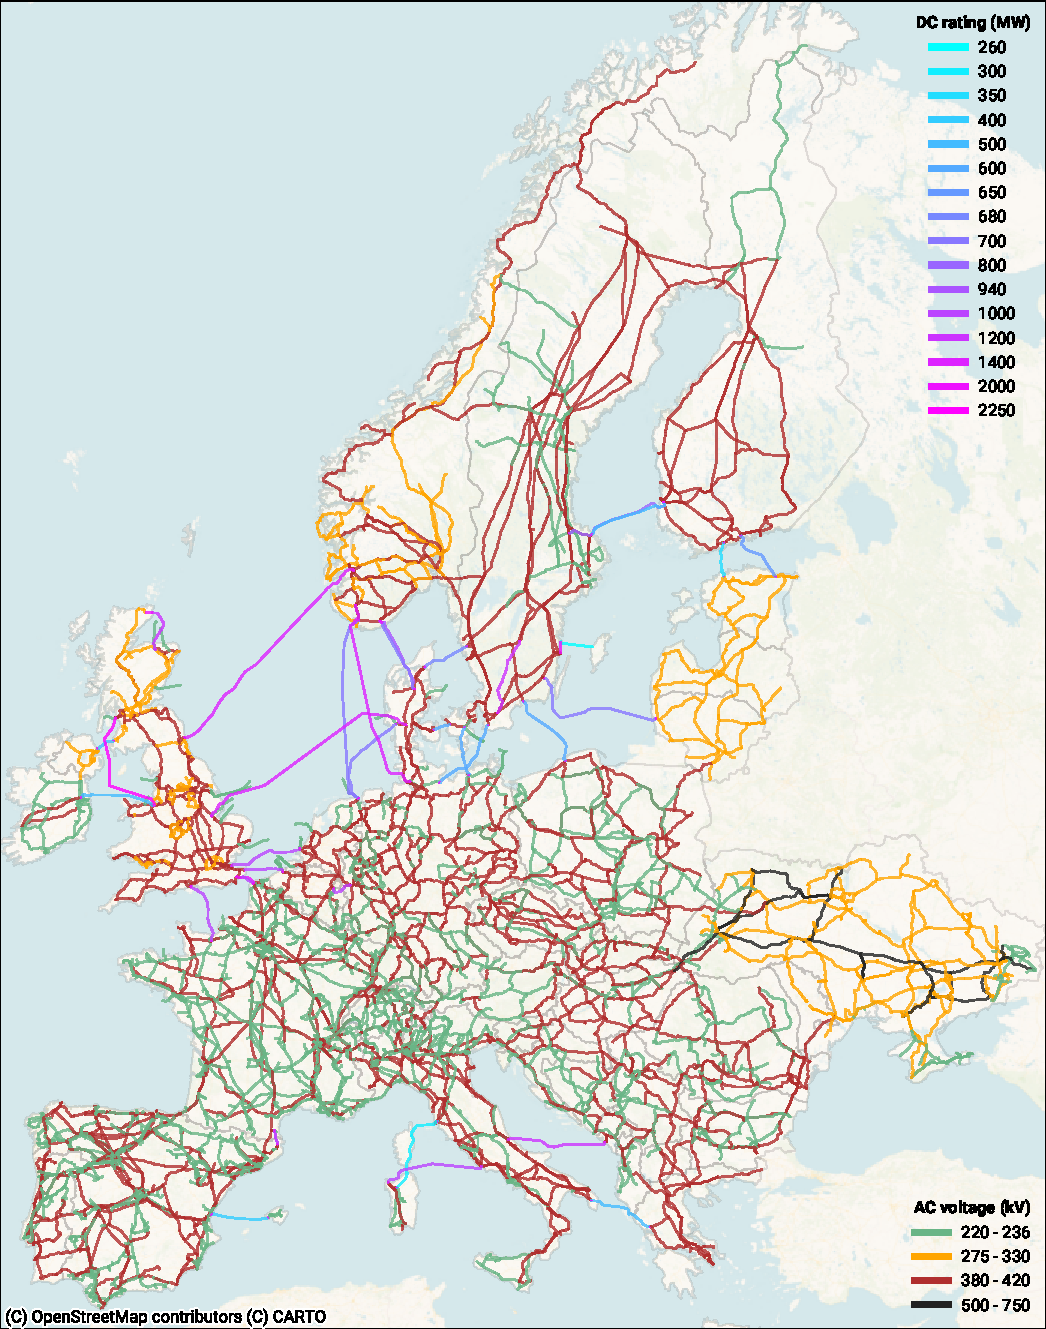
\includegraphics[width=0.99\textwidth] {figures/fig_osm_map.pdf}
    \caption{Map of the \acrshort{osm}-based European high-voltage grid. \textit{This map was generated using the grid dataset provided with this publication. \autocite{xiongPrebuiltElectricityNetwork2024}}}
    \label{fig:osm_map}
\end{figure}


\newpage
\newpage
\section*{Technical Validation}
% \pdfcomment{This section presents any experiments or analyses that are needed to support the technical quality of the dataset. This section may be supported by figures and tables, as needed. This is a required section; authors must present information justifying the reliability of their data.}
We perform two validation steps for assessing the quality of the dataset. First, we compare the dataset with official inventory statistics provided by \acrshort{entsoe}. Second, we compare the results of an representative PyPSA-Eur model instance based on the two high-voltage grid datasets: OSM (presented in \ref{fig:osm_map}) and an extract from the online ENTSO-E map using GridKit tool (referred to as ‘ENTSO-E map’).\autocite{wiegmansGridKitExtractENTSOE2016} This network is currently being used by numerous PyPSA-Eur users, and is hence a good reference for comparison. In Figure \ref{fig:osm_vs_50Hertz_sgm}, we further provide a comparison between a geo-referenced, official dataset by 50Hertz\autocite{50hertzStaticGridModel2022} and the \acrshort{osm}-based grid of the region, respectively.

\subsection*{Comparison with \acrshort{entsoe} statistics and map}
Based on \acrshort{entsoe}'s 2023 inventory of transmission,\autocite{entso-eInventoryTransmission20232024} we first compare the total route (a) and circuit lengths (b) of \acrshort{ac} lines and cables on a per country level (Figure \ref{fig:bar_lengths}.). Note that the inventory does not include all statistics for each country, i.e. route lengths are missing for Bosnia and Herzegovina, Switzerland, and Great Britain, while circuit lengths are missing for Montenegro and North Macedonia. While Ukraine and the Republic of Moldova have joined \acrshort{entsoe} on 1 January 2024 and 22 November 2023 as full and observing members, respectively, their inventory are not yet included in the dataset. For these two countries, we take reference data from third party sources.\autocite{cigrePowerSystemUkraine2018,globaldataTopFiveTransmission2023,moldelectricaTechnicalEconomicIndicators2023}

\begin{figure}[!htbp]
    \centering
    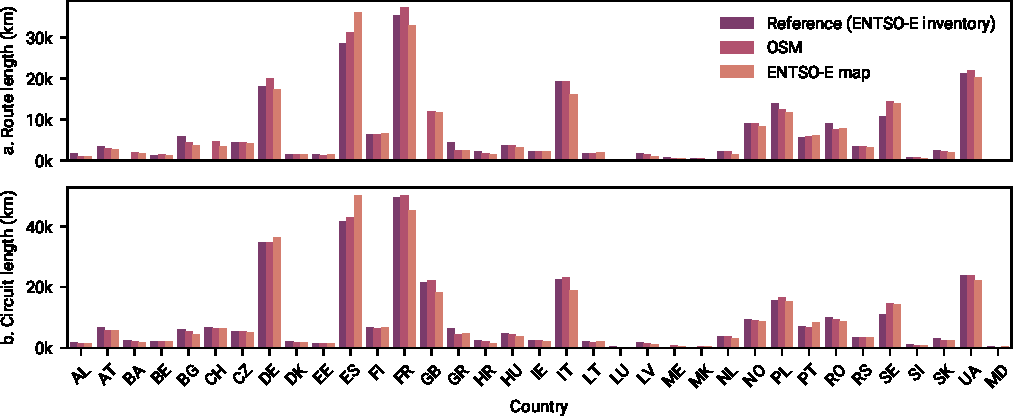
\includegraphics{figures/fig_bar_lengths.pdf}
    \caption{Comparison of total route and circuit lengths per country.}
    \label{fig:bar_lengths}
\end{figure}

We find that our transmission grid based on \gls{osm} data is in agreement with the \acrshort{entsoe} inventory. Calculating the Pearson correlation coeffficient for both route and circuit lengths between the official statistics and the respective transmission grid representations, we see an overall improvement from the \acrshort{entsoe} map ($\rho_{routes} = 0.9497$ and $\rho_{circuits} = 0.9862$) to \gls{osm} ($\rho_{routes} = 0.9636$ and $\rho_{circuits} = 0.9980$) in the reproduction of the high-voltage grid (\SI{220}{\kilo\volt} to \SI{750}{\kilo\volt}). One of the key reasons for these improvements is the much higher level of geographic detail of lines and cables in the \gls{osm}-based transmission grid compared to the stylised lines on \acrshort{entsoe}'s interactive map. We observe larger discrepancies for Sweden, where both transmission grid representations seem to overestimate the total lengths of the inventory.

\begin{figure}[!htbp]
    \centering
    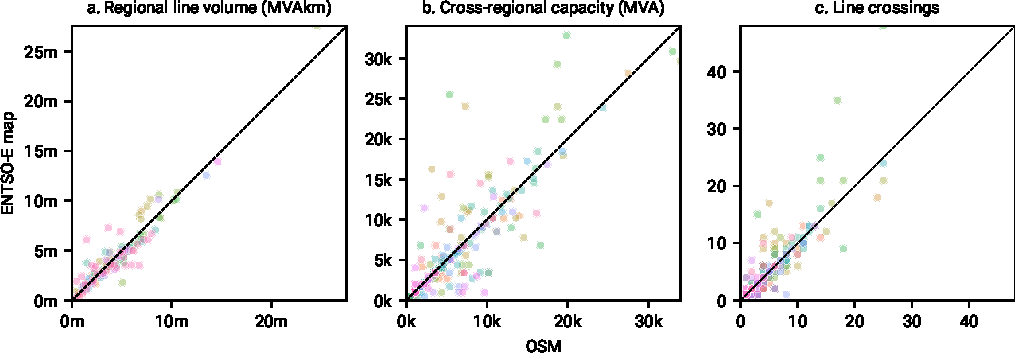
\includegraphics{figures/fig_scatter_joined.pdf}
    \caption{Comparison of line volume per NUTS1 region $-$ Colors represent individual countries. \textit{Line volume is the product of the nominal capacity and the length, summed over all lines within the region.}}
    \label{fig:scatter_joined}
\end{figure}

As another validation step, we compare the total line volume on NUTS1 region level (Figure \ref{fig:scatter_joined}.a). Here we see strong similarities between the \acrshort{osm}-based and the extracted transmission grid of the \acrshort{entsoe} map, with few outliers ($\rho_{MVAkm} = 0.9484$). While a higher geospatial resolution of lines of the \gls{osm}-based transmission grid may contribute to the increase in line volume on average, we calculate $S_{nom}^{AC}$ using the more differentiated voltage levels given in the \gls{osm} data (see Table \ref{tab:s_nom}) as opposed to the clustered voltage levels given in the \acrshort{entsoe} map, i.e. \SI{220}{\kilo\volt}, 300 to \SI{330}{\kilo\volt}, 380 to \SI{400}{\kilo\volt}, \SI{500}{\kilo\volt}, and \SI{750}{\kilo\volt}. This may lead to a more accurate representation of the line volume in the \gls{osm}-based transmission grid.

To assess the transmission capacity across regions, we compare the capacity (Figure \ref{fig:scatter_joined}.b) and number of line crossings (Figure \ref{fig:scatter_joined}.c) per NUTS1 border (Figure \ref{fig:scatter_joined}.b). While the two transmission grids strongly correlate, we observe notable differences at individual borders ($\rho_{MVA} = 0.8491$), the same is true for the absolute number of line crossings ($\rho_{crossings} = 0.8573$). Due to different quality in geospatial information contained in both transmission grid representations, buses in one may be offset (or not even exist) in the other. Stronger outliers can primarily be traced back to buses close to NUTS1 borders (Figure \ref{fig:scatter_joined}.b). Notable outliers are located in Spain (light green), in Ukraine (pink), and southwestern parts of Germany (ocher). The reasons for discrepancies can be manifold, e.g. due to differences in exact locations of boundary nodes, missing, outdated or wrong data. In the case of Spain, the main reason for the large discrepancy lies in the representation of the high-voltage grid in and around the Madrid area, where the \acrshort{entsoe} map is stylised for clarity. A comparison with an official map provided by the National Geographic Institute of Spain\autocite{institutogeograficonacionalEnergiaMapaRed2016} confirms the \gls{osm} topology to be more accurate.

\subsection*{Comparison of model results}
In order to assess the impact of the new transmission grid representation, we compare the results of a representative PyPSA-Eur model run based on the \gls{osm} dataset to a run based on the \acrshort{entsoe} map which is currently being used in PyPSA-Eur. \autocite{horschPyPSAEurOpenOptimisation2018} Note that the results shown in this publication are based on version 0.3 of the released prebuilt high-voltage grid representation on Zenodo.\autocite{xiongPrebuiltElectricityNetwork2024} We use the same model setup and input data in both model runs, except for the grid representation. We focus on the electricity sector, taking techno-economic assumptions projected for the year 2030. We allow for capacity expansion in renewable energy as well as gas-fired generation capacities. To narrow down the effect of the transmission grid, we do not allow for grid expansion and disable dynamic line rating. We set the carbon price to 100 \euro{} per tonne of \ce{CO2} emitted.

\begin{figure}[!htbp]
    \centering
    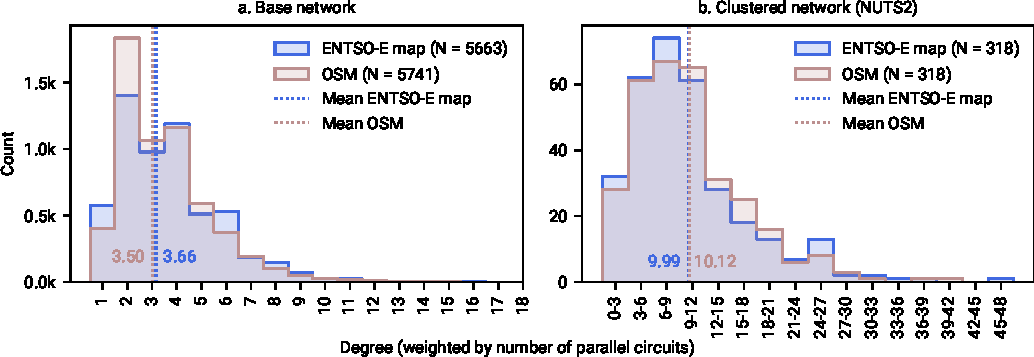
\includegraphics{figures/fig_hist_degree_nuts2.pdf}
    \caption{Comparison of the weighted degree distribution in both transmission grid representations before and after clustering (NUTS2). \textit{Ukraine at geoBoundaries\autocite{runfolaGeoBoundariesGlobalDatabase2020} administration level 1, Moldova in full bus resolution. A comparison at NUTS3 resolution is provided in Figure \ref{fig:hist_degree_nuts3}.}}
    \label{fig:hist_degree_nuts2}
\end{figure}

As the number and exact locations of buses differ, we cluster the networks to make them comparable (N = 318 regions/buses). In energy system modelling, clustering is often motivated by the spatial reduction of the optimisation problem. While oftentimes clustering algorithms based on grid topology or resource class are used, \autocite{frysztackiComparisonClusteringMethods2022} we are interested in the regional differences of the two grid representations. As such, we map the buses of both grids to clusters based on administrative boundaries, i.e. NUTS2. For non-NUTS countries such as Ukraine, we use the administration level 1 (geoBoundaries\autocite{runfolaGeoBoundariesGlobalDatabase2020}) and for Moldova we keep the full high-voltage substation resolution, i.e. 8 nodes. This yields 318 regions/buses for each of the clustered high-voltage grids, respectively. Note that the clustering process in PyPSA-Eur involves a transformation of all transmission lines and cables to the default voltage level of \SI{380}{\kilo\volt}. We then run the model at hourly resolution of the year 2030, yielding 8760 time steps. 

Figure \ref{fig:hist_degree_nuts2} compares the weighted degree distribution for the two network topologies. We weight the degree by the number of parallel circuits (Eq. \ref{eq:weighted_degree}) to account for potential different representations of lines and links connecting the same two buses (e.g., single lines with multiple number of circuits or multiple lines with single circuits). If \( G = (V, E) \) is a weighted graph with vertex set \( V \) (buses) and edge set \( E \) (lines, links, converters, and transformers), and each edge \( e \in E \) has a weight \( w(e) \), then the weighted degree of a vertex \( v \in V \) is given by:

% begin math environment

\begin{equation}
    d_w(v) = \sum_{e \in \text{IncidentEdges}(v)} w(e)
    \label{eq:weighted_degree}
\end{equation}

where \( \text{IncidentEdges}(v) \) is the set of edges incident to \( v \). We find that the two base networks have a similar weighted degree distribution (Pearson correlation coefficient $\rho_{degree,base} = 0.8518$). Notably, the \acrshort{osm}-based transmission grid demonstrates a higher number of buses with degree 2. Clustering the two networks before running the optimisation problem will increase the Pearson correlation coefficient to $\rho_{clustered,base} = 0.8769$ (using unbinned data), $\rho_{clustered,base} = 0.9937$ (using binned data) --- indicating that at NUTS2 resolution, the two networks are very similar in terms of connectivity and adequately represent the real grid.

\begin{figure}[!htbp]
    \centering
    \includegraphics{figures/fig_results_sidebyside.pdf}
    \caption{Regional dispatch, line utilisation and curtailment. \textit{A map comparing nominal ratings of the two clustered grids is provided in the Figure \ref{fig:results_sidebyside_capacity}.}}
    \label{fig:results_sidebyside}
\end{figure}

We solve the two optimisation problems on a high-performance cluster (AMD EPYC 7543 32-Core processor) using up to \SI{130}{\giga\byte} of memory. Each problem takes up to 274 iterations to converge, translating into more than 18 hours. Running the model for the two transmission grid representations, we find that regional results align closely, including the dispatch of generation assets, utilisation of lines and curtailment (Figure \ref{fig:results_sidebyside}). This is also true for the aggregated picture (Table \ref{tab:results}). Total system costs drop from 312.94 bn. \euro{} in the \acrshort{entsoe} map based run to 311.7 bn. € in the \acrshort{osm}-based optimisation, corresponding to mere \SI{0.40}{\percent} in difference. The higher weighted degree for both the base and clustered \acrshort{osm}-based high-voltage grid (Figure \ref{fig:hist_degree_nuts2}) indicate a higher topological connectivity, potentially translating into higher degrees of freedom in the optimisation problem compared to the \acrshort{entsoe} map based run. This is confirmed when we look into i) the line and link utilisation and ii) compare the investments. Since aggregate statistics over a continental area can be deceiving (smooth out errors), we show the differences in regional generation, line and link utilisation as well as curtailment in Figure \ref{fig:results_delta}. Here, we can clearly see that the high-voltage grid in \acrshort{osm} is higher utilised than its \acrshort{entsoe} map based counterpart. We can also observe that the \acrshort{entsoe} map based model compensates by investing more into generation (especially decentral, semi-circles in the bottom half) and storage capacities, i.e. +\SI{4.9}{\giga\watt} in solar photovoltaics, +\SI{4.8}{\giga\watt} in onshore wind, +\SI{1.1}{\giga\watt} in offshore wind (\acrshort{ac}), and +\SI{2.4}{\giga\watt} in battery storage. In the \acrshort{osm}-based model run, we see a slightly stronger build-out of \acrshort{dc} connected offshore wind (+\SI{2.7}{\giga\watt}). We also provide an overview of average electricity prices, CAPEX and OPEX at nodal level in Figure \ref{fig:results_cost_scatter}.

\begin{table}[!htbp]
    \centering
    \csvreader[
        tabular=|r|c|c|c|c|c|,
        table head=\hline & 
        \makecell{\textbf{System costs} \\ (bn. \euro{}/a)} &
        \makecell{\textbf{CAPEX} \\ (bn. \euro{}/a)} &
        \makecell{\textbf{OPEX} \\ (bn. \euro{})/a} &
        \makecell{\textbf{Curtailment} \\ (\SI{}{\tera\watt\hour}/a)} &
        \makecell{\textbf{Generation} \\ (\SI{}{\tera\watt\hour}/a)}
        \\\hline,
        late after line=\\\hline,
        head to column names
    ]{datatables/tab_results.csv}{}%
    { 
        \ifthenelse{\equal{\thecsvrow}{1}}{ENTSO-E map}{%
        \ifthenelse{\equal{\thecsvrow}{2}}{OSM}{%
        \ifthenelse{\equal{\thecsvrow}{3}}{ Delta (\SI{}{\percent})}{}}}& 
        \csvcolii & \csvcoliii & \csvcoliv & \csvcolv & \csvcolvi
    }
    \caption{Comparison of key result metrics between \acrshort{entsoe} map and \acrshort{osm}-based transmission grid.}
    \label{tab:results}
\end{table}

Bottlenecks in both model runs are located in the same regions, contributing to an annual curtailment in the range of \SI{2176}{\tera\watt\hour} to \SI{2178}{\tera\watt\hour}. More prominent differences in line utilisation are visible in Norway and Poland from North to South, in the western region of Ukraine, southern and central Spain around the Madrid area, as well as southern Italy. 

Overall, the results of the two model runs are very similar, indicating that i) both grids seem to adequately represent reality and ii) the \gls{osm}-based transmission grid is a suitable replacement for the \acrshort{entsoe} map based grid. The higher utilisation of the \gls{osm}-based transmission grid is in line with the higher topological connectivity of the network. The differences in the investment decisions are marginal and can be attributed to the differences in grid topology.

We have shown that the dataset is in good agreement with official statistics and the \acrshort{entsoe} map, and the results of a representative PyPSA-Eur model instance based on the two high-voltage grid datasets are very similar. Its core strengths lie in the high level of geographic detail and the continuous updates to the \gls{osm} database in combination with a strong PyPSA-Eur user base. The workflow is completely transparent and the data is provided openly. While we cannot guarantee the correctness of the data, as only \acrshortpl{tso} have access to the real grid data, we believe that the dataset provides the best publicly available representation of the European high-voltage grid.

\newpage
\begin{figure}[!htbp]
    \centering
    \includegraphics{figures/fig_results_delta.pdf}
    \caption{Regional dispatch, line utilisation and curtailment. \textit{Blue indicates an increase in curtailment or line utilisation from the \acrshort{entsoe} map to the \gls{osm}-based transmission grid, while red indicates a decrease. For full transparency, note that this map shows an outer join of all transmission grid elements, including lines and links that are not present in the other network.}}
    \label{fig:results_delta}
\end{figure}

\newpage

\section*{Usage Notes}
% The Usage Notes should contain brief instructions to assist other researchers with reuse of the data. This may include discussion of software packages that are suitable for analysing the assay data files, suggested downstream processing steps (e.g. normalization, etc.), or tips for integrating or comparing the data records with other datasets. Authors are encouraged to provide code, programs or data-processing workflows if they may help others understand or use the data. Please see our code availability policy for advice on supplying custom code alongside Data Descriptor manuscripts.

% For studies involving privacy or safety controls on public access to the data, this section should describe in detail these controls, including how authors can apply to access the data, what criteria will be used to determine who may access the data, and any limitations on data use. 

The published dataset is provided under the \gls{odbl} 1.0 licence. Geoinformation is encoded in the WGS84 (EPSG:4326) coordinate system. Although the dataset and workflow are provided as part of PyPSA-Eur, they are also suitable for a wide range of other applications, including network analyses, power flow calculations, as well as an input for other energy energy system models and frameworks. Note that further validation and testing is needed for purposes outside the original scope of this work. 

\begin{itemize}
    \item In order to reproduce the network with the latest \gls{osm} data, the configuration file `config.yaml': needs to be set to \colorcode{base_network = `osm-prebuilt'} and the command \colorcode{snakemake base_network -call} needs to be executed.
    \item To rebuild the network from scratch, this setting can be changed to \colorcode{base_network = `osm-raw'}, followed by the command \colorcode{snakemake prepare_osm_network_release -call}. 
    \item Per default, buses within the perimeter of a \SI{5000}{\meter} radius are merged together. This value can be changed in the script, however this may change the topological connectedness of the obtained network. 
    \item Networks can also be built for specific countries, regions or a subset of the countries within PyPSA-Eur by setting list of \colorcode{countries} the configuration file.
\end{itemize}
To abide to the fair use policy of the \acrshort{osm} Overpass turbo \acrshort{api}, we kindly encourage users to download the prebuilt network topology from the Zenodo repository and only rebuild the network, if necessary. We would further like to encourage readers to actively contribute to the \acrshort{osm} database.


\section*{Code availability}
% For all studies using custom code in the generation or processing of datasets, a statement must be included under the heading "Code availability", indicating whether and how the code can be accessed, including any restrictions to access. This section should also include information on the versions of any software used, if relevant, and any specific variables or parameters used to generate, test, or process the current dataset. 

The code to replicate the entire workflow and dataset is provided as part of PyPSA-Eur and released as free software under the MIT licence. Different licences and terms of use may apply to the underlying input data.
\begin{itemize}
    \item PyPSA-Eur \autocite{horschPyPSAEurOpenOptimisation2018} on GitHub: \\ \href{https://github.com/pypsa/pypsa-eur}{https://github.com/pypsa/pypsa-eur}
    \item Version 0.3 of the prebuilt network\autocite{xiongPrebuiltElectricityNetwork2024} based on \acrshort{osm} data can be retrieved via the Zenodo repository. This link will also point to future updates: \\ \href{https://zenodo.org/records/13358976}{https://zenodo.org/records/13358976}
\end{itemize}

\bibliography{osm-for-pypsa-eur}

% \noindent LaTeX formats citations and references automatically using the bibliography records in your .bib file, which you can edit via the project menu. Use the cite command for an inline citation, e.g. \cite{Kaufman2020, Figueredo:2009dg, Babichev2002, behringer2014manipulating}. For data citations of datasets uploaded to e.g. \emph{figshare}, please use the \verb|howpublished| option in the bib entry to specify the platform and the link, as in the \verb|Hao:gidmaps:2014| example in the sample bibliography file. For journal articles, DOIs should be included for works in press that do not yet have volume or page numbers. For other journal articles, DOIs should be included uniformly for all articles or not at all. We recommend that you encode all DOIs in your bibtex database as full URLs, e.g. https://doi.org/10.1007/s12110-009-9068-2.

\section*{Acknowledgements} % (not compulsory)
% Acknowledgements should be brief, and should not include thanks to anonymous referees and editors, or effusive comments. Grant or contribution numbers may be acknowledged.
The authors would like to thank the \gls{osm} community for their tremendous motivation and efforts in providing the data underlying this work. Further, the authors would like to thank the PyPSA-Earth community for setting the groundwork and initiating the move to grid data based on \gls{osm}. Last but not least, the authors would like thank Ekaterina Fedotova and Emmanuel Bolarinwa for early substantial developments and validations in integrating \acrshort{osm} into PyPSA-Earth and Philipp Glaum for technical sparring and support. Map data copyrighted OpenStreetMap contributors and available from \href{https://www.openstreetmap.org}{https://www.openstreetmap.org}. 

This work was supported by the German Federal Ministry for Economic Affairs and Climate Action (BMWK) under Grant No. 03EI4083A (RESILIENT) and Italian Ministry of University and Research (MUR) CUP I53C23002650007 (RESILIENT). This project has been funded by partners of the CETPartnership (https://cetpartnership.eu/) through the Joint Call 2022. As such, this project has received funding from the European Union's Horizon Europe research and innovation programme under grant agreement no. 101069750.

\section*{Author contributions statement}
B.X. -- Conceptualisation, Data curation, Methodology, Software/Programming, Model building and validation, Visualisation, Writing -- original draft, review and editing. 
D.F. -- Conceptualisation, Software/Programming, Writing -- review and editing.
F.N. -- Conceptualisation, Discussion, Writing -- review and editing.
I.R. -- Discussion, Writing -- review and editing.
T.B. -- Supervision, Writing -- review and editing.

% B.X., F.N. and T.B. conceptualised the project. B.X. and D.F. wrote wrote key data processing scripts. B.X. conducted data collection, model building, data processing and model validation work. All authors discussed the results, contributed to writing the manuscript, and commented on the manuscript at all stages in the review process.
% A.A. conceived the experiment(s), A.A. and B.A. conducted the experiment(s), C.A. and D.A. analysed the results. All authors reviewed the manuscript. 

\section*{Competing interests} % (mandatory statement)
% \pdfcomment{The corresponding author is responsible for providing a competing interests statement on behalf of all authors of the paper. This statement must be included in the submitted article file.}
The authors declare no competing interests.

\newpage
\section*{Figures \& Tables}

% \pdfcomment{Figures, tables, and their legends, should be included at the end of the document. Figures and tables can be referenced in \LaTeX{} using the ref command, e.g. Figure \ref{fig:stream} and Table \ref{tab:example}. 

% Authors are encouraged to provide one or more tables that provide basic information on the main ‘inputs’ to the study (e.g. samples, participants, or information sources) and the main data outputs of the study. Tables in the manuscript should generally not be used to present primary data (i.e. measurements). Tables containing primary data should be submitted to an appropriate data repository.

% Tables may be provided within the \LaTeX{} document or as separate files (tab-delimited text or Excel files). Legends, where needed, should be included here. Generally, a Data Descriptor should have fewer than ten Tables, but more may be allowed when needed. Tables may be of any size, but only Tables which fit onto a single printed page will be included in the PDF version of the article (up to a maximum of three). 

% Due to typesetting constraints, tables that do not fit onto a single A4 page cannot be included in the PDF version of the article and will be made available in the online version only. Any such tables must be labelled in the text as ‘Online-only’ tables and numbered separately from the main table list e.g. ‘Table 1, Table 2, Online-only Table 1’ etc.}


\begin{table}[!htbp]
    \centering
    \begin{tabular}{|p{0.25\textwidth}|p{0.71\textwidth}|}
    \hline
    \textbf{Grid element} & \textbf{Overpass turbo query}  \\
    \hline
    \acrshort{ac} power lines and cables & \colorcode{way[`power'=`line']} and \colorcode{way[`power'=`cable']} \\
    \hline
    \acrshort{dc} links & \colorcode{relation[`route'=`power'][`frequency'=`0']} \\
    \hline
    substations & \colorcode{way[`power'=`substation']} and \colorcode{relation[`power'=`substation']} \\
    \hline
    \end{tabular}
    \caption{Overpass turbo queries used to extract the high-voltage grid elements from \acrshort{osm}.}
    \label{tab:overpass_queries}
\end{table}

\begin{table}[!htbp]
    \centering
    \begin{tabular}{|p{2.5cm}|p{2.6cm}|p{3.5cm}|p{3cm}|p{1.5cm}|p{2cm}|}
    \hline
    \textbf{Project} & \textbf{Regional scope} & \textbf{Tools/data} & \textbf{Last update} & \textbf{Geo\-referenced} & \textbf{Data \newline published} \\
    \hline
    50Hertz static grid model\autocite{50hertzStaticGridModel2022} & Germany (50Hertz control area) & based on asset inventory & April 2022 \newline (updated once a year) & Yes & Yes \\
    \hline
    ELMOD\autocite{egererElectricitySectorData2014} & Europe & ENTSO-E interactive map\autocite{entso-eENTSOETransmissionSystem} plus manual changes & January 2014 \newline (data not published) & Yes & No \\
    \hline
    ELMOD-DE\autocite{egererOpenSourceElectricity2016} & Germany & VDE, \acrshort{tso} maps, and \acrshort{osm} & March 2016
     \newline (single release) & Yes & Yes (not reproducible) \\
    \hline
    Hutcheon \& Bialek\autocite{hutcheonUpdatedValidatedPower2013} & Europe (UCTE plus Balkan region) & PowerWorld model & June 2013 \newline (updated once) &  No & Yes (not reproducible) \\
    \hline
    JAO static grid model\autocite{jaoStaticGridModel2023} & CORE capacity calculation region & based on CORE \acrshort{tso} asset inventory & April 2024 \newline (updated frequently) &  No & Yes \\
    \hline
    PyPSA-Eur\autocite{horschPyPSAEurOpenOptimisation2018} & Europe & ENTSO-E interactive map\autocite{entso-eENTSOETransmissionSystem} using GridKit\autocite{wiegmansGridKitExtractENTSOE2016} plus manual changes& January 2022 \newline (updated once) &  Yes & Yes (reproduction complex) \\
    \hline
    osmTGmod \autocite{OsmTGmodDocumentation2017} & Germany & \acrshort{osm} using Osmosis (SQL and Java)\autocite{wiegmansGridKitExtractENTSOE2016} & November 2017 \newline (single release) &  Yes & Yes (reproduction complex)\\
    \hline
    SciGrid (Power) \autocite{medjroubiOpenDataPower2017} & Europe, Germany & \acrshort{osm} using GridKit\autocite{wiegmansGridKitExtractENTSOE2016} & November 2015 \newline (updated once) & Yes & Yes (reproduction complex)\\
    \hline
    \bfseries This publication & Europe & \acrshort{osm} using Overpass turbo \acrshort{api} and Python & August 2024 \newline (updated frequently) &  Yes & Yes \autocite{xiongPrebuiltElectricityNetwork2024} (reproducible)\\
    \hline
    \end{tabular}
    \caption{Notable projects and datasets modelling the high-voltage grid in Europe (alphabetical order). \textit{Note that the specific regional scope referring to `Europe' may vary across the listed projects. A comparison of our dataset with the 50Hertz static grid model is shown in Figure \ref{fig:osm_vs_50Hertz_sgm}.}}
    \label{tab:network_projects}
\end{table}

\newpage
\begin{table}[!htbp]
    \centering
    \csvreader[
        tabular=|C{2.5cm}|C{4.8cm}|C{1.4cm}|C{1.4cm}|C{1.2cm}|C{1.2cm}|C{1.9cm}|, % Specify column widths
        table head=\hline 
        \bfseries \makecell{\acrshort{osm} relation \\ identifier} & 
        \makecell{\bfseries \acrshort{dc} project name \\ (sorted alphabetically)} & 
        \bfseries From & 
        \bfseries To & 
        \makecell{\textbf{Voltage} \\(\SI{}{\kilo\volt})} & 
        \makecell{\textbf{Rating} \\(\SI{}{\mega\watt})} & 
        \makecell{\textbf{Calc. length} \\(\SI{}{\kilo\meter})} 
        \\\hline,
        late after line=\\\hline,
        head to column names
    ]{datatables/dc_links.csv}{}%
    {\csvcoli & \csvcolii & \csvcoliii & \csvcoliv & \csvcolv & \csvcolvi & \csvcolvii}

    \caption{List of \acrshort{dc} projects in the \acrshort{osm}-based transmission grid. \textit{Note that \acrshort{osm} relation identifiers are unique and persistent as long as the object is not deleted. Projects can be directly accessed via the \acrshort{osm} website by clicking on their respective relation identifier in the table.}}
    \label{tab:dc_links}
\end{table}


\newpage
% S_nom after mapped to pandapower standard type library
\begin{table}[!htbp]
    \centering 
    \csvreader[
        tabular=|c|c|r|r|r|r|,
        table head=\hline\bfseries $\bm{U_{nom}^{OSM}}$ (\SI{}{\kilo\volt}) & \bfseries Line type & \bfseries $\bm{I_{nom}^
        {pandapower}}$ (\SI{}{\ampere}) & \bfseries $\bm{n_{circuits}}$ & \bfseries $\bm{S_{nom}^{AC}}$ (\SI{}{\mega\volt\ampere}) & \bfseries Total route length (\SI{}{\kilo\meter}) \\\hline,
        late after line=\\\hline,
        head to column names
    ]{datatables/tab_s_nom.csv}{}%
    {\csvcoli & \csvcolii & \csvcoliii & \csvcoliv & \csvcolv & \csvcolvi}
    \caption{\label{tab:s_nom} Nominal capacities in the \acrshort{osm} base network  \acrshort{ac} lines and cables to pandapower standard type library.}
\end{table}

\begin{figure}[!htbp]
    \centering
    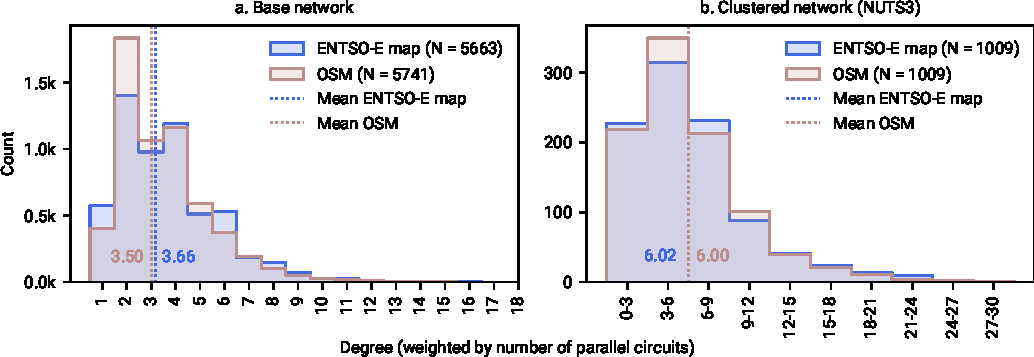
\includegraphics{figures/fig_hist_degree_nuts3.pdf}
    \caption{Comparison of the weighted degree distribution in both networks before and after clustering (NUTS3). \textit{Ukraine at geoBoundaries\autocite{runfolaGeoBoundariesGlobalDatabase2020} administration level 1, Moldova in full bus resolution.}}
    \label{fig:hist_degree_nuts3}
\end{figure}

\newpage
\begin{figure}[!htbp]
    \centering
    \includegraphics{figures/fig_results_sidebyside_capacity.pdf}
    \caption{Clustered \acrshort{ac} line capacities, \acrshort{dc} link nominal ratings, and optimal generation capacities.}
    \label{fig:results_sidebyside_capacity}
\end{figure}

\begin{figure}[!htbp]
    \centering
    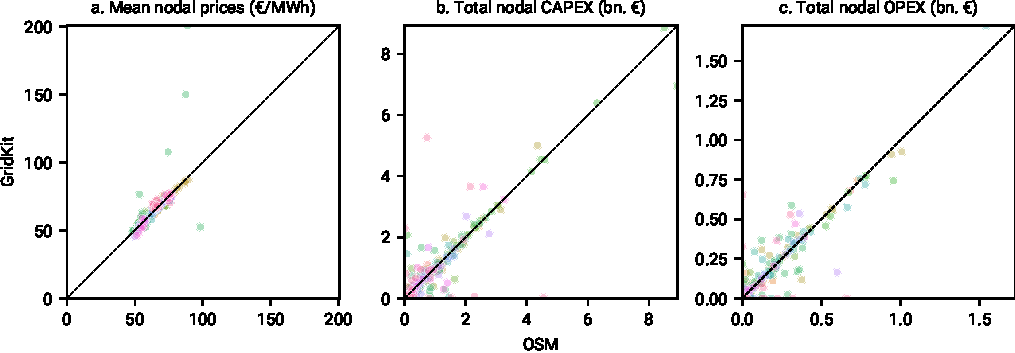
\includegraphics{figures/fig_results_cost_scatter.pdf}
    \caption{Comparison of nodal prices, capital expenditures (CAPEX) and operational expenditures (OPEX). \textit{Outliers nodal prices (a): Great-Britain (green). Outliers nodal CAPEX (b): Ukraine (pink).}}
    \label{fig:results_cost_scatter}
\end{figure}

\begin{figure}[!htbp]
    \centering
    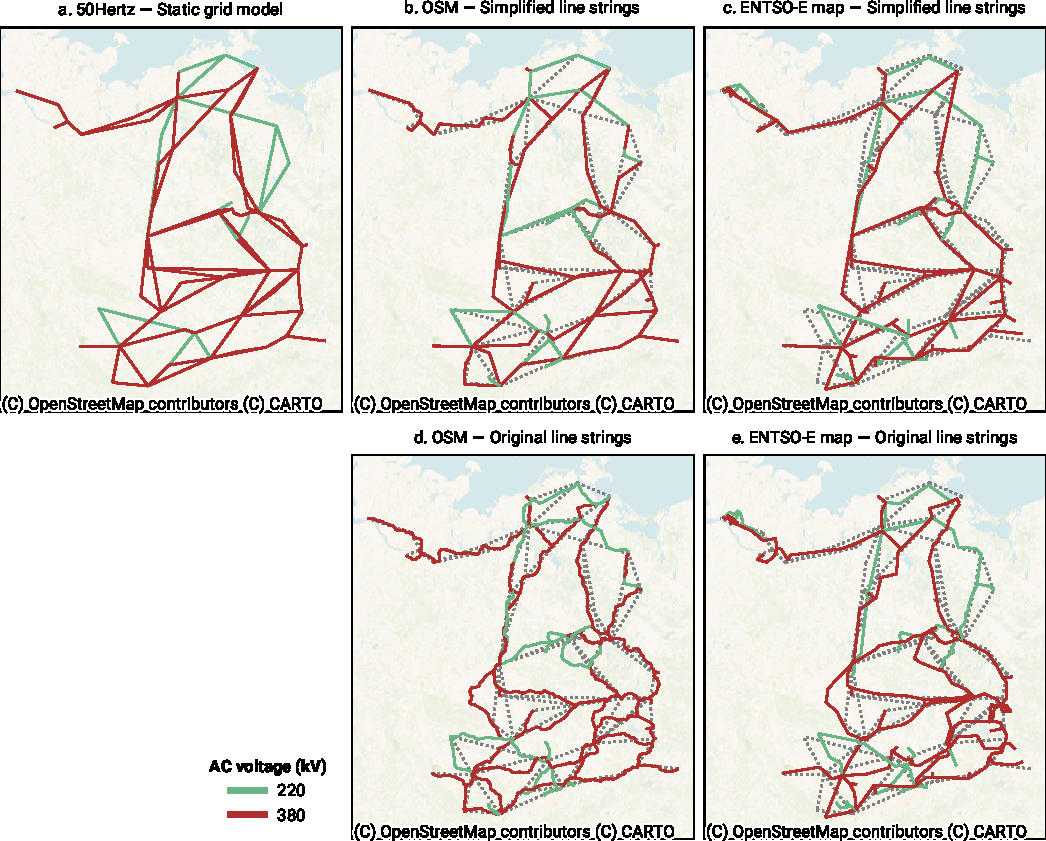
\includegraphics{figures/fig_osm_vs_50Hertz_sgm.pdf}
    \caption{Comparison of \acrshort{osm} and \acrshort{entsoe} map-based transmission grid with reference 50Hertz static grid model.\autocite{50hertzStaticGridModel2022} \textit{Dashed grey lines underneath show the 50Hertz static grid model for comparative purposes. Note that the geospatial data is provided in simplified, point-to-point form, only. Many of the dashed grey lines are also included in the \acrshort{osm} or \acrshort{entsoe} map-based grid representations, however, intermediary buses exists along the line. As such, in their simplification they are not simplified to the level of the 50Hertz static grid model.}}
    \label{fig:osm_vs_50Hertz_sgm}
\end{figure}

\newpage
\begin{figure}[!htbp]
    \centering
    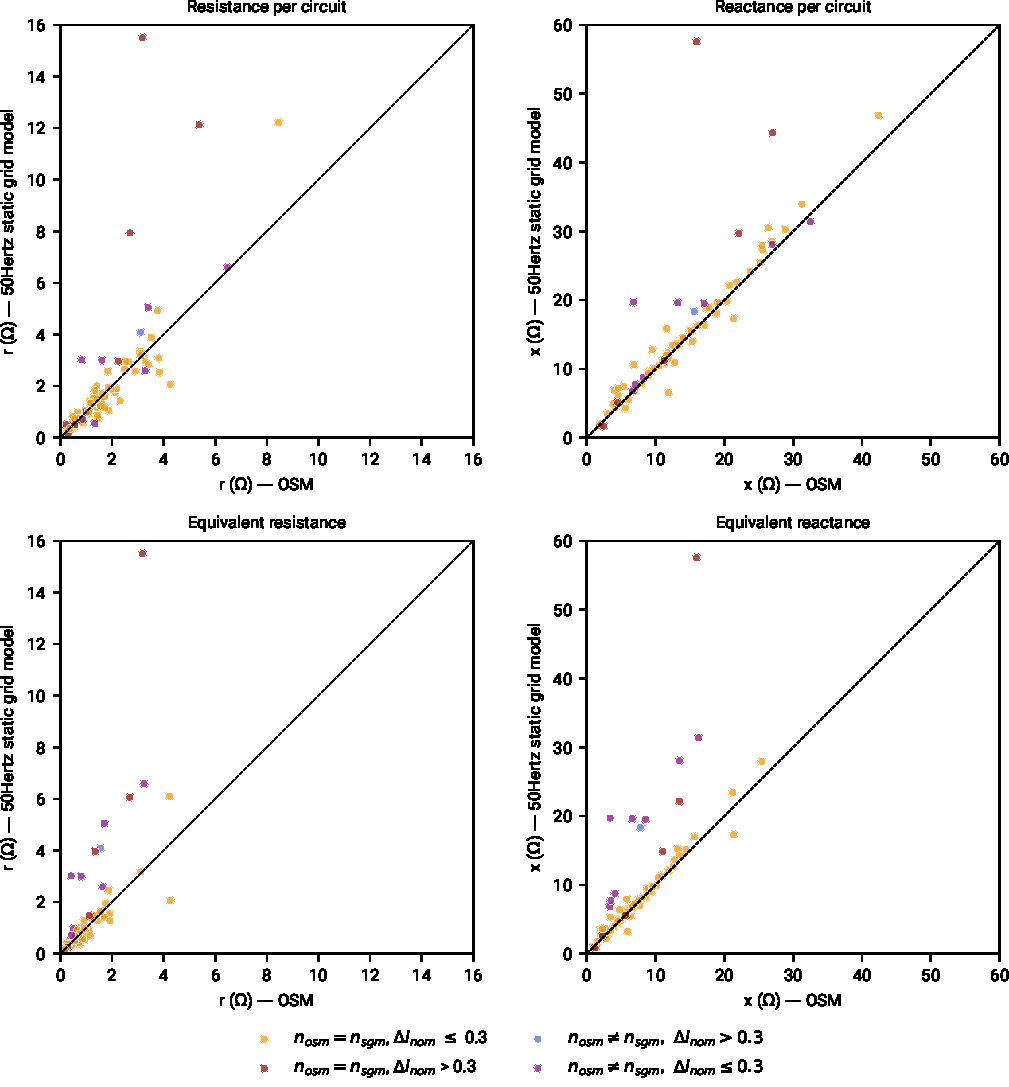
\includegraphics{figures/fig_scatter_reactance_resistance.pdf}
    \caption{Comparison of \acrshort{ac} line/cable resistance and reactance between the \acrshort{osm}-based transmission grid and reference 50Hertz static grid model.\autocite{50hertzStaticGridModel2022} \textit{$n_{osm}$ and $n_{sgm}$ refer to the number of parallel circuits for a distinct line in each network, while $\Delta i_{nom} = \frac{|i_{nom, osm} - i_{nom, sgm}|}{i_{nom,sgm}}$ refers to the relative change in underlying nominal current.}}
    \label{fig:scatter_reactance_resistance}
\end{figure}

Figure \ref{fig:scatter_reactance_resistance} was generated by mapping \acrshort{ac} lines and cables of the \acrshort{osm}-based transmission grid to the 50Hertz static grid model (SGM) using \acrshort{osm} tags and SGM names (right join). Note that this data explains \SI{4475}{\kilo\meter} of \SI{5126}{\kilo\meter} in route length, as not all lines could mapped. For \SI{79}{\percent} of the data, using pandapower's standard line types\autocite{thurnerPandapowerOpenSourcePython2018} for calculating the resistance and reactance comes close to official data in the SGM (orange). Purple data points a discrepance primarily due to unequal number of parallel circuits in both datasets (SGM data larger by factor 2). Red and blue data points indicate that underlying line types are entirely different. This is the case for some lines where SGM e.g. has a newer \SI{380}{\kilo\volt} (allowing higher higher currents) or weaker \SI{220}{\kilo\volt} line type.




\end{document}